% 
% 
% 

\subsection{Software}

Se entiende como Software a todo soporte lógico e intangible necesario que hacen posible la realización de tareas especificas. Según el estándar 729 de la IEEE, se entiende como  el conjunto de programas, procedimientos, reglas, documentación y datos asociados que forman parte de las operaciones de un sistema de cómputo. Entre los componentes lógicos se puede hacer mención de aplicaciones informáticas, el sistema operativo que permite que los programas funcionen correctamente y los programas de interfaz de usuario. \\

Por lo general, el software se escribe en lenguajes de programación de alto nivel, es decir que son herramientas de programación fáciles y eficientes para los programadores debido a su semejanza al lenguaje natural. Por su parte los sistemas de cómputo ejecutan estos programas en lenguaje máquina. La traducción entre estos lenguajes se realiza mediante un compilador que se encarga de ``traducir'' las instrucciones.

\subsubsection{Clasificación}
\begin{itemize}

    \item \textbf{Sistema: }
    Es el tipo de software de alto nivel que separa las acciones del usuario en comparación de las acciones de bajo nivel que debe ejecutar el sistema de cómputo con respecto a su memoria, procesador, etc.
    
    \item \textbf{Programación: }
   Son las herramientas que le facilitan al programador programar los algoritmos informáticos mediante lenguajes de programación de manera aplicada. A grosso modo poseen Editores de texto, compiladores, intérpretes y entornos de desarrollo que cuentan con interfaces gráficas para el usuario.
    
\end{itemize}

\subsubsection{Codificación de algoritmos en OSS}

El Software de Código Abierto OSS (Open Source Software) es un concepto relativamente reciente que abarca un modelo de desarrollo de software basado en colaboración abierta en Internet, donde un propietario de software permite a los usuarios utilizar, cambiar y redistribuir el software para cualquier propósito. \cite{Defopensource}.

El proceso para  diseñar software se logra con el objetivo de idear la forma en que las acciones se realizarán en el marco de un proyecto para solventar una necesidad en particular. Hoy en día se considera programación al proceso de escritura de algoritmos computacionales mediante un editor de texto o herramienta integrada como los lenguajes de programación entre los que se encuentran Python, C y C++.

Los algoritmos son un conjunto de instrucciones o reglas predefinidas de manera ordenada que permiten llevar a cabo una actividad mediante pasos consecutivos secuenciales o paralelos de manera no ambigua para poder realizar una actividad \cite{algoritmo}. Los algoritmos computacionales son algoritmos más sofisticados y precisos que permiten aprovechar las nuevas tecnologías y que al depender de una memoria limitada deben ser lo mas optimizados posible para que puedan procesar grandes cantidades de datos con capacidades finitas y generalmente a bajo costo.

% =========================================================
    
% =========================================================


\subsection{Data Clustering}

\subsubsection{Bases de datos digitales}
Es un conjunto de datos interrelacionados y almacenados de forma ordenada y sistemática (Ver Figura \ref{databasepng}) para un uso posterior\cite{database}. Debido al desarrollo tecnológico de la informática y la electrónica, estas bases de datos suelen ser digitales y por lo general se almacenan en la nube (Cloud). Por otra parte, es considerado un modelo de almacenamiento de datos basado en redes de computadoras, donde los datos están alojados en espacios de almacenamiento virtualizados \cite{cloud}.

	\begin{figure}[H]
		\begin{center}
			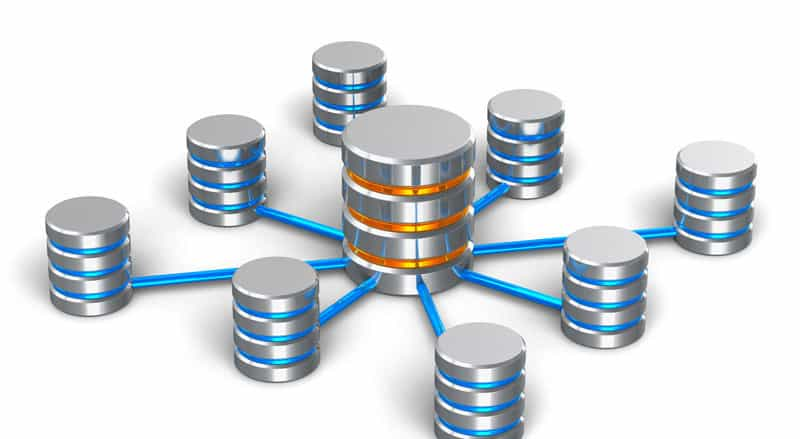
\includegraphics[scale=0.5]{img/databasepng.png}
		\end{center}
	\caption{Base de datos. Tomada de \cite{googlepics}. \label{databasepng}}
	\end{figure}

% \subsubsection{Cloud}

% %%% Tek

% La nube, también denominada como ``Cloud Storage" (Ver Figura \ref{cloudpng}), se refiere tanto a las aplicaciones entregadas como servicios a través de Internet y el software del hardware y sistemas en los centros de datos que proporcionan estos servicios \cite{cloud2}.
% 	\begin{figure}[H]
% 	\begin{center}
% 		
\includegraphics[scale=0.45]{img/cloud.png}
% 	\end{center}
% 	\caption{Almacenamiento en nube. Tomada de \cite{googlepics}. \label{cloudpng}}
% 	\end{figure}
